\documentclass[10pt]{article}

\usepackage{fullpage}
\usepackage{setspace}
\usepackage{parskip}
\usepackage{titlesec}
\usepackage{placeins}
\usepackage{xcolor}
\usepackage{breakcites}
\usepackage{lineno}





\PassOptionsToPackage{hyphens}{url}
\usepackage[colorlinks = true,
            linkcolor = blue,
            urlcolor  = blue,
            citecolor = blue,
            anchorcolor = blue]{hyperref}
\usepackage{etoolbox}
\makeatletter
\patchcmd\@combinedblfloats{\box\@outputbox}{\unvbox\@outputbox}{}{%
  \errmessage{\noexpand\@combinedblfloats could not be patched}%
}%
\makeatother


\usepackage[round]{natbib}
\let\cite\citep




\renewenvironment{abstract}
  {{\bfseries\noindent{\abstractname}\par\nobreak}\footnotesize}
  {\bigskip}

\renewenvironment{quote}
  {\begin{tabular}{|p{13cm}}}
  {\end{tabular}}

\titlespacing{\section}{0pt}{*3}{*1}
\titlespacing{\subsection}{0pt}{*2}{*0.5}
\titlespacing{\subsubsection}{0pt}{*1.5}{0pt}


\usepackage{authblk}


\usepackage{graphicx}
\usepackage[space]{grffile}
\usepackage{latexsym}
\usepackage{textcomp}
\usepackage{longtable}
\usepackage{tabulary}
\usepackage{booktabs,array,multirow}
\usepackage{amsfonts,amsmath,amssymb}
\providecommand\citet{\cite}
\providecommand\citep{\cite}
\providecommand\citealt{\cite}
% You can conditionalize code for latexml or normal latex using this.
\newif\iflatexml\latexmlfalse
\providecommand{\tightlist}{\setlength{\itemsep}{0pt}\setlength{\parskip}{0pt}}%

\AtBeginDocument{\DeclareGraphicsExtensions{.pdf,.PDF,.eps,.EPS,.png,.PNG,.tif,.TIF,.jpg,.JPG,.jpeg,.JPEG}}

\usepackage[utf8]{inputenc}
\usepackage[english]{babel}








\begin{document}

\title{Review on INArxiv preprint:~K-Means Method for Clustering Water Quality
Status on The Rivers of Banjarmasin~}



\author[1]{Dasapta Erwin Irawan}%
\author[2]{PREreview Team}%
\affil[1]{Institut Teknologi Bandung}%
\affil[2]{Affiliation not available}%


\vspace{-1em}



  \date{\today}


\begingroup
\let\center\flushleft
\let\endcenter\endflushleft
\maketitle
\endgroup





\selectlanguage{english}
\begin{abstract}
This is a preprint journal club review of~K-Means Method for Clustering
Water Quality Status on The Rivers of Banjarmasin
by~\href{https://osf.io/a59hw/}{Tien Zubaidah}~and Nieke Karnaningroem.
The preprint was originally posted on~\href{http://inarxiv.id}{INArxiv}
on December 21, 2017 (link:~\url{https://osf.io/g6wkp/}). The article is
now in review in the ARPN Journal of Engineering and Applied Sciences
(submitted December 20, 2017).

\par\null

\textbf{Original abstract:~}The surface river water quality in
Banjarmasin city tends to decline constantly as the result of direct and
indirect waste disposal from various human activities along the river
body. This study aimed to determine the vulnerability points against
pollution in the rivers of Banjarmasin using clustering techniques with
K-means algorithm. The parameters observed include Biological Oxygen
Demand (BOD), Chemical Oxygen Demand (COD), Total Suspend Solid (TSS)
and Dissolved Oxygen (DO). The data were collected at eight water
monitoring stations on various rivers in Banjarmasin city. With the
K-means method, four water quality status were clustered. The result
showed that 6 stations observed during the period April to October 2016
were categorized into the heavy polluted cluster with major pollution
point of sources came from the domestic and industrial activities.%
\end{abstract}%




\section*{Short review}

{\label{419658}}

\subsection*{Introduction}

{\label{737266}}

Yang terhormat Tim Penulis ( Ibu Tien dan Ibu Nieke)~

\par\null

Pertama-tama saya mengucapkan terima kasih telah menggunakan layanan
INArxiv. Semoga layanan kami ini dapat memaksimumkan pengembangan
risetnya. Ulasan ini juga menjadi bukti bahwa salah satu manfaat
mengunggah naskah preprint adalah mendapatkan umpan balik dari rekan
sebidang. Saat ini cara untuk memberikan ulasanpun tidak konvensional
seperti dulu, melalui editor sebuah jurnal, melainkan bisa melalui
saluran seperti blog pribadi, e-mail, atau bahkan ulasan publik melalui
laman \emph{journal club} seperti ini.

\par\null

\begin{quote}
Reviewing has been extensively developed from conventional way,
via~journal editor, to a more open and personal way directly to the
author, via personal email, personal blogpost, or via a journal club
like this review.~ ~
\end{quote}

\par\null

Saya tertarik dengan naskah berikut ini. Sejalan dengan fokus riset saya
di bidang hidrogeologi. Makalah ini dengan sangat baik telah menjelaskan
alur riset dengan sangat baik. Hasilnyapun telah merepresentasikan
tujuan riset.~Penurunan kualitas air sungai sudah menjadi masalah di
mana-mana, terutama di kota besar di dunia. Berbagai metode memang sudah
seharusnya digunakan untuk memerangi hal tersebut. Salah satunya adalah
metode karakterisasi kualitas air dengan teknik~\emph{K-Means
clustering}.

\par\null

\begin{quote}
River contamination has been a major problem in big cities in Indonesia
and also the world
\end{quote}

\par\null

\subsection*{\texorpdfstring{Pentingnya \emph{reproducibility} dalam
sains}{Pentingnya reproducibility dalam sains}}

{\label{411520}}

Namun demikian perkenankan saya menambahkan sedikit catatan untuk
makalahnya. Di dunia saat ini sedang berkembang konsep sains terbuka
(open science) yang salah satunya mendorong setiap makalah perlu
memiliki struktur untuk dapat direproduksi. Reproduksi (produksi ulang)
sangat penting dalam dunia saintifik, karena setiap output riset harus
dapat dianalisis ulang oleh pihak lain untuk menjamin validitasnya.
Makalah yang reproducible juga memiliki peluang disitat lebih besar. Dua
komponen penting untuk mendukung ini adalah: data mentah dan metode
analisis yang rinci.

\par\null

Yang saya pahami, sering terjadi penulis terkendala oleh jumlah halaman
maksimum atau jumlah kata maksimum untuk dapat lebih rinci menjelaskan
dua hal di atas. Untuk data mentah akan bagus kalau diunggah. Dalam
kasus makalah ini sedang direview oleh sebuah jurnal, maka data mentah
dapat diunggah sekaligus dalam halaman preprint ini. Ibu dapat melakukan
``edit preprint'' dan mengunggah file data mentah dalam berbagai format
(xls, csv, dll). Kemudian dalam naskah disunting dengan menambahkan
tautan preprint di atas untuk mengarahkan pembaca yang berminat untuk
mengetahui data. Berikut ini saya sampaikan diagram spektrum dalam
\emph{reproducibility} \cite{theory}.~

\par\null

\begin{quote}
Reproducibility is very important to ensure the validity of a research
(or paper)
\end{quote}

\par\null\par\null\selectlanguage{english}
\begin{figure}[h!]
\begin{center}
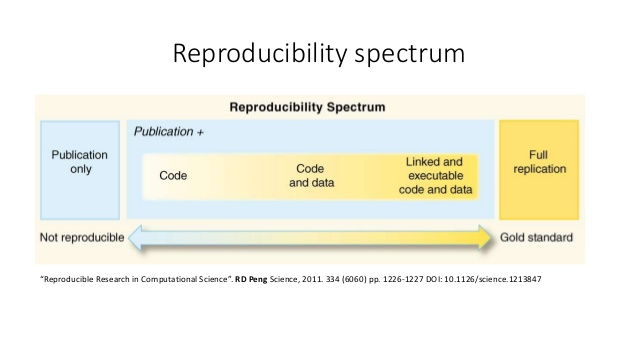
\includegraphics[width=0.70\columnwidth]{figures/reproducible-research-theory-8-638/reproducible-research-theory-8-638}
\caption{{Spektrum \emph{reproducibility}~\protect\cite{Peng_2011}
{\label{114879}}%
}}
\end{center}
\end{figure}

\par\null

Bila ada pembaca yang berminat mereproduksi makalah atau akan
menggunakan data mentahnya, maka ia dapat melakukan ``forking''
(pencabangan proyek) ini dengan mudah untuk masuk ke dalam proyek OSF
ybs. Kemudian ybs dapat melakukan berbagai analisis sesuai keperluannya
tanpa mengubah file-file yang ada dalam proyek ibu.

\par\null

\begin{quote}
Someone who wishes to reproduce an OSF-based preprint could easily
``fork'' the original document to do his/her own analysis
\end{quote}

\par\null

Untuk analisis, Ibu dapat menjelaskan tahapan rinci pengolahan data.
Akan lebih bagus kalau piranti lunak yang digunakan berbasis teks
(\emph{command line}), dengan demikian, ibu cukup melampirkan file kode
sebagai file pendukung makalah secara terpisah (lihat gambar di atas).

\par\null

\subsection*{Peluang pengembangan dalam
analisis}

{\label{473265}}

Dalam analisis disajikan beberapa penyebab mengapa terjadi perubahan
kluster pada bulan yang berbeda, namun penjelasan baru memasukkan
variabel curah hujan. Akan lebih baik bila makalah ini dikembangkan
dengan mengaitkan perubahan tersebut dengan perubahan tata guna lahan
atau kontribusi output air tanah yang mengalir menuju sungai. Alasan
saya mengemukaan ini adalah BOD atau COD biasanya berkaitan dengan
limbah domestik atau peternakan yang membuang limbang langsung ke sungai
tanpa pengolahan terlebih dahulu, yang mana ini sering terjadi di
Indonesia. Perubahan tata guna lahan dari lahan terbuka menjadi
perumahan bisa jadi salah satu indikasi.

~

Alasan saya yang kedua adalah, pada Sungai Cikapundung
\cite{Darul_2015}, Sungai Ciliwung \cite{Irawan_2014}, dan
Cisadane~\cite{julian2016} serta anak-anak sungai di Gunung Ciremai
\cite{Irawan_2009}, sangat mungkin ada kontribusi air tanah ke sungai.
Rembesan air dari akuifer ini juga dapat membawa zat polutan terutama
bila aliran air tanah bersinggungan dengan titik-titik sumber
kontaminasi organik, misal \emph{septic tank}.~ ~

\par\null

Pengamatan secara time series pada beberapa tahun dengan melibatkan
analisis citra satelit \cite{oktavia2017,k2017} akan sangat bagus. Kekuatan
analisis spasial dapat melengkapi analisis statistik yang telah
dilakukan oleh penulis.

\par\null

\subsection*{Peluang kolaborasi}

{\label{473265}}

Yang ketiga, saya berminat untuk melakukan kolaborasi menulis paper
bersama Ibu dan rekan-rekan yang lain yang mungkin berminat. Usulan
saya, kita gabungkan data mentah dari berbagai lokasi dan dianalisis
secara bersama untuk mengetahui kesamaan atau perbedaan karakter
diantaranya. Secara spasial saya juga ingin membuat clustering dengan
metode hirarkis yang lebih visual. Bila itu digabungkan dengan analisis
spasial, maka akan lebih bermanfaat bagi pihak pengelola daerah.
Strategi pengelolaan air bisa sangat bergantung kepada hasil analisis
tersebut.~

\par\null

\begin{quote}
With this review, I hereby also propose to make a potential
collaboration~
\end{quote}

\par\null

Demikian kurang lebih komentar dan juga proposal saya agar dapat
dimanfaatkan bila ada kesempatan.

\par\null

Salam, Erwin (\href{http://osf.io/he3j7}{osf.io/he3j7})

\href{http://www.itb.ac.id}{Institut Teknologi Bandung}

\href{http://dasaptaerwin.net}{Personal blog}

\selectlanguage{english}
\FloatBarrier
\bibliographystyle{plainnat}
\bibliography{bibliography/converted_to_latex.bib%
}

\end{document}

